\chapter{Problem Decomposition and Analysis} \label{chapter:ch2_analysis}

In this chapter we will analyze the goals of this thesis and derive requirements for our system. We will then analyze different approaches of meeting these requirements, compare them to each other, and select an approach best suited to our goals and requirements. 

\section{Target tasks and their requirements} \label{sec:ch2_analysis_tasks_and_requirements}

Let us first re-state the goals we want to achieve with our system for reference:
\begin{goals}
  \item \label{an_goal:1} Explore and validate programming of cooperative robots directly in the real workspace by defining robot motions and tool actions using spatial, AR-inspired inputs, as an alternative to traditional teach pendant, offline programming, and hand-guiding workflows.
  \item \label{an_goal:2} Provide an extensible system where task-oriented use cases can be implemented as plugins that reuse the same acquisition/execution infrastructure.
  \item \label{an_goal:3} Demonstrate the approach on a real robot with representative use cases for a material-handling task (pick-and-place) and a trajectory-centric task (seam welding), and evaluate the benefits and limitations of spatial authoring for these tasks.
\end{goals}

First, we will define the requirements for the system based on the use cases we want to implement. The two use cases mentioned in goal \ref{an_goal:3} are a material-handling task (\emph{pick-and-place}) and a trajectory-centric task (\emph{seam welding}). 

Our system should also support the addition of new use cases (goal~\ref{an_goal:2}), so we will outline some potential future use cases and see if the requirements derived from our main use cases are sufficient to support them as well. 

One example of a future use case is a \emph{painting task}, where the goal is to uniformly paint a selected face of an object using a spray gun. In addition, the system should be capable of expressing traditional robot motion primitives (e.g., moving to a point or along a path). While such primitives are not the main focus of our work, their compatibility with the proposed input architecture is relevant.

The ability to support both these additional tasks and the primary use cases does not constitute a formal proof of generality; rather, it serves as a \emph{plausibility check} and a concrete data point indicating that the proposed requirements and abstractions are sufficiently expressive to cover a broader class of tasks, including ones not explicitly targeted during system design.

\subsection{Pick-and-place} \label{subsec:ch2_analysis_pick_and_place}

One way to implement a \emph{pick-and-place} task is the following:
\begin{enumerate*}[label=(\arabic*)]
    \item \emph{scan the scene} to find the object to be picked (we also need to know which object to pick),
    \item \emph{calculate the grasp pose} (the detected position of the object is not necessarily the same as the grasp pose),
    \item \emph{move to the grasp pose},
    \item \emph{close the gripper},
    \item \emph{move to the release pose} without crashing into anything,
    \item \emph{open the gripper}, and
    \item \emph{move away}, for example, to a safe home position.
\end{enumerate*}

This gives us several task-specific requirements:
\begin{enumerate*}[label=(\roman*)]
    \item the system needs to be able to capture the scene and detect objects in it, \label{req:scene_detection}
    \item the system needs to be able to calculate the grasp pose based on the detected object, \label{req:grasp_calculation}
    \item the user needs to define the object type to be picked, and \label{req:object_type}
    \item the user needs to define the release pose. \label{req:release_pose}
\end{enumerate*}

Therefore the system will need to be able to provide at least \emph{scene detection} logic (covers requirement \ref{req:scene_detection}) and a spatial \emph{6D input interface} (requirement \ref{req:release_pose}). Requirement \ref{req:object_type} can be fulfilled either by a simple UI element (e.g. dropdown) or by spatial input as well --- given that we already plan to support a \emph{6D input interface}, we can also use it for object type selection too. Finally requirement \ref{req:grasp_calculation} can be fulfilled either on the use case plugin level (plugin will calculate the grasp pose based on the detected object) or even from the user input (user selects the object with a 6D input, we can also consider the selection pose as the grasp pose).

\subsection{Seam welding} \label{subsec:ch2_analysis_seam_welding}

One way to implement a \emph{seam welding} task is the following:
\begin{enumerate*}[label=(\arabic*)]
    \item \emph{approach the seam} to be welded (usually not the start of the seam, but a point close to it),
    \item \emph{approach the start of the seam},
    \item \emph{start welding},
    \item \emph{move along the seam} while welding,
    \item \emph{stop welding} at the end of the seam, and
    \item \emph{move away}, for example, to a safe home position.
\end{enumerate*}

This gives us the following task-specific requirements:
\begin{enumerate*}[label=(\roman*)]
    \item the user needs to define the approach pose (a point close to the start of the seam), \label{req:approach_pose}
    \item the user needs to define the seam (either as a linear segment --- start and end points --- or as a trajectory), and \label{req:seam_definition}
    \item the user needs to define the welding parameters (e.g. welding speed, welding power, weaving settings). \label{req:welding_parameters}
\end{enumerate*}

To fulfill these requirements, we could use the same \emph{6D input interface} as for the pick-and-place use case --- the user can select the approach pose (fulfilling requirement \ref{req:approach_pose}) and then define the seam by either selecting the start and end points of the seam or by defining a trajectory along the seam (requirement \ref{req:seam_definition}).

However this approach would depend heavily on the precision of the \emph{6D input interface}. Therefore we could instead first use the \emph{scene detection} logic to detect objects within the scene and then use use case specific logic to detect possible seams between the detected objects --- the user would then still use the \emph{6D input interface} to enter a trajectory representing the seam, however the system would align the user's input to the closest detected seam (requirement \ref{req:seam_definition}). The approach pose (requirement \ref{req:approach_pose}) could be automatically defined by the use case as a point at a certain distance from the start of the seam along the seam normal. Finally, the welding parameters (requirement \ref{req:welding_parameters}) could be defined by a simple UI element (with reasonable defaults).

\subsection{System requirements} \label{subsec:ch2_analysis_system_requirements}

Subsections \ref{subsec:ch2_analysis_pick_and_place} and \ref{subsec:ch2_analysis_seam_welding} give us the following system requirements:
\begin{requirements}
    \item \emph{6D input interface} for defining poses and trajectories (both in 6D; that is, with position and orientation) in the workspace. While extreme precision is not strictly required --- since use-case-specific logic can refine the user input with the help of the scene data --- higher input precision is nevertheless preferable, as it simplifies downstream processing, improves alignment robustness, and better supports future use cases with tighter accuracy requirements. \label{req:6D_input_interface}
    \item \emph{scene detection} logic that can detect objects in the scene and provide their poses. The precision requirements for the scene detection are higher than for the 6D input interface, because we use the detected objects to refine the user input. \label{req:scene_detection_logic}
    \item \emph{UI} for defining non-spatial parameters (e.g. object type for pick-and-place, welding parameters for seam welding). \label{req:ui}
\end{requirements}

Beyond the requirements directly derived from the use cases, we also have some more general requirements:
\begin{requirements}[resume]
    \item \emph{UI} also has to support selection of the use case to be programmed, visualization of the created program, and confirmation of the programming. This requirement is not directly derived from the use cases, but it is necessary for a complete system that can be used by end-users. \label{req:ui_use_case_selection}
    \item \emph{robot communication interface} that allows the use cases to move the robot and control its tool, and that can support multiple robot brands/models to ensure broader applicability. \label{req:robot_communication_interface}
    \item \emph{use case plugin support} that allows the addition of new use cases as plugins, reusing the same input and execution infrastructure outlined in the previous requirements. \label{req:use_case_plugin_support}
\end{requirements}

\subsection{Coverage of Additional Use Cases}

The requirements outlined in \autoref{subsec:ch2_analysis_system_requirements} are sufficient to cover the additional use cases mentioned in \autoref{sec:ch2_analysis_tasks_and_requirements}. 

For example, the \emph{painting task} can be implemented using the \emph{6D input interface} to select the face to be painted as a 6D pose or a trajectory circling the the face. The requested face can then be chosen by the use case logic as the face closest to the user input. The \emph{UI} can be used to define painting parameters (e.g. paint flow rate, spray pattern) and the use case can then generate the appropriate robot trajectory.

Similarly, traditional robot motion primitives can also be implemented using the same \emph{6D input interface} for defining target poses or paths. This use would require higher precision and lower noise of the input, particularly for defining paths, which further emphasizes the importance of a high-quality \emph{6D input interface}. At the same time, a use case may apply smoothing or refinement to the user-provided path, which can partially relax the precision requirements on the input.

\section{Requirement-driven design decisions}

Based on the requirements outline in \autoref{subsec:ch2_analysis_system_requirements}, we decompose the system into the following five components as illustrated in \autoref{fig:ch2_analysis__base_components}:
\begin{enumerate*}[label=(\roman*)]
    \item 6D input interface, 
    \item scene detection,
    \item robot execution interface,
    \item UI, and 
    \item use case plugin support.
\end{enumerate*}

\begin{figure}
  \centering
  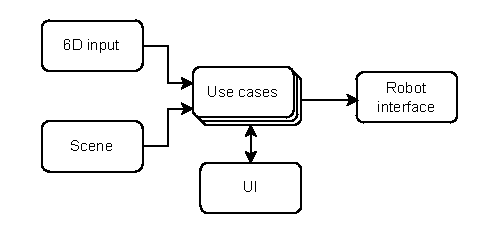
\includegraphics{img/ch2_analysis/base_components__valid.pdf}
  \caption{Base components of our system.}
  \label{fig:ch2_analysis__base_components}
\end{figure}

For each component we compare feasible approaches and select one for this thesis.

\subsection{6D input interface}

As stated in requirement \ref{req:6D_input_interface}, our system needs to provide \emph{6D input} (position and orientation) for defining poses and trajectories in the real workspace. High precision is not a strict requirement for our two use cases, because use case logic can refine user input using scene data, but higher stability and lower jitter are still desirable --- they simplify downstream processing and keep the interface usable for potential future tasks.

When selecting an input approach, we consider:
\begin{enumerate*}[label=(\roman*)]
    \item required hardware and calibration effort,
    \item tracking quality (noise/jitter, occlusion sensitivity, and latency),
    \item integration complexity, and
    \item \emph{intent signalling} --- how the user indicates when to capture a pose or start/stop sampling a trajectory.
\end{enumerate*}

We consider three candidate approaches:
\begin{enumerate*}[label=(\roman*)]
    \item \emph{hand tracking}, where the user's hand is the input device,
    \item \emph{VR/AR controllers}, using existing VR/AR hardware, and
    \item \emph{camera-based marker tracking}, where the user holds a tool with a known marker tracked by an external camera.
\end{enumerate*}

\paragraph{Hand tracking.}
Hand tracking is an attractive option because it is intuitive and does not require a dedicated held tool. It can be implemented using open-source solutions such as MediaPipe \cite{MediaPipeRoot} (also used by Vysocký et al.\ \cite{Vysocky2023}) or via commercial ecosystems such as the Meta Quest headset or Leap Motion. Meta Reality Labs also reports several recent research systems for hand tracking on headset devices \cite{FB_research, FB__UmeTrack, FB__MEgATrack, FB__ElasticHandTrack}.
However, robust 6D interaction in our setting requires not only a plausible hand pose, but also sufficiently stable spatial position and orientation for selecting poses and drawing trajectories. With a single RGB camera (e.g., MediaPipe), metric depth can only be estimated, which is typically not accurate enough for precise workspace authoring. Multi-camera setups or RGB-D sensors can mitigate this (as in \cite{Vysocky2023}), but at the cost of additional calibration effort and system complexity. Additionally, reported accuracy limitations for gesture-based robot path definition \cite{Vysocky2023} make hand tracking a risky default for our use case.
A related idea by Zhang et al.\ \cite{Zhang2023} improves robustness for surface-following by using an RGB-D-T camera and thermal cues to infer contact on the object surface, but this does not directly generalize to trajectories in free space.

Hand tracking also complicates \emph{intent signalling}, because there is no explicit hardware trigger for pose capture or trajectory start/stop. This can be implemented using gestures, but gesture recognition can be error-prone and may conflict with reliable orientation estimation (e.g., pointing provides a clear direction, while pinch-like gestures can be less stable and can be triggered accidentally). Tracking quality can also degrade under occlusions and changing lighting conditions.

One could attempt to restrict hand tracking to 2D interaction and use scene data to infer intent (e.g., selecting a seam on a surface). While such a design could work for some surface-bound tasks, it does not generalize to cases where target poses are not located on a visible surface (e.g., a free-space release pose in pick-and-place). Therefore, we only consider fully 3D hand tracking as a candidate here.


\paragraph{VR/AR controllers.} 
VR/AR controllers offer accurate, low-latency 6D tracking and typically provide explicit buttons, which makes intent signalling (capture pose or start/stop sampling a trajectory) straightforward. The downside is that this approach requires dedicated hardware and depends strongly on the tracking stack and APIs provided by the manufacturer.

\paragraph{Camera-based marker tracking.}
Marker tracking is a widely used approach in AR pipelines: a known marker is detected in the camera image and its 6D pose is estimated. Compared to hand tracking, it can be simpler to implement, works with a single camera, and can provide sufficiently stable input for our authoring tasks. Since the user already holds a tool with the marker, we can also add an explicit trigger (e.g., a button), making intent signalling straightforward. The main limitation is that precision depends strongly on practical factors such as camera quality, marker size, viewing distance, lighting, and occlusion. In general, camera-only pipelines may introduce latency depending on camera exposure, frame rate, and processing, but they avoid some of the ambiguity inherent in single-camera hand tracking.

The D-Point pen \cite{dpoint_github} illustrates this category (camera-based marker tracking combined with an IMU), although replication reports \cite{dpoint_issues} indicate that achieved precision can be sensitive to implementation and hardware choices.

\begin{table}[t]
\centering
\caption{Comparison of candidate 6D input approaches.}
\label{tab:6D_input_comparison}

\small 

\begin{tabular}{l l c c c c}
\toprule
Approach & Hardware & Cost & Accuracy & Intuitiveness & Complexity \\
\midrule
Hand tracking &
2+ cameras &
Medium &
Low &
High &
High\textsuperscript{a} \\

VR/AR &
VR headset &
High &
High &
Medium &
Medium\textsuperscript{b} \\

Marker tracking &
Camera &
Low &
Medium &
Medium &
Low\textsuperscript{c} \\
\bottomrule
\end{tabular}

\vspace{0.4em}
\footnotesize
\emph{Note:}
\textsuperscript{a} Multi-camera calibration; robust hand tracking algorithms; non-trivial intent signaling. \\
\textsuperscript{b} Depends on manufacturer stack/APIs; intent is easy via buttons. \\
\textsuperscript{c} Marker detection widely available; intent is easy via tool button.
\end{table}

Since both demonstrative use cases require repeated capture of stable poses and short trajectories near objects, we prioritize robustness and predictable capture over maximum intuitiveness.

Table~\ref{tab:6D_input_comparison} summarizes the trade-offs. Given our constraints, marker tracking provides the best balance of implementation effort and usable tracking quality for pose and trajectory authoring, while keeping hardware requirements low. Therefore, we select a camera-based marker tracking approach for the 6D input interface in this thesis. At the same time, we keep the input interface modular to allow substituting alternative 6D input sources (e.g., hand tracking or VR controllers) in future work.



\newpage

\xxx{The next chapter will start with scene input requirement - pen tracking + scene + camera }

\xxx{Analysis of requirements}
    \xxx{6D input interface}
    \xxx{scene detection}
    \xxx{camera trade-offs}
    \xxx{Robot interface - what exactly do we require (move J, move L, move A, move T and status and that actually means just move J is requried and the rest can be implemented on top of it in the interface. The replacability of the robot interface is important -> another motivation for a modular architecture.)}
    \xxx{UI - select usecase, confirm, visualziation. what did we pick and why.}
    \xxx{Usecase plugin support - here instead do modular architecfure (and that automatically satisfier R6 while also significnatly helping with the rest - we can excahnge etc. This will be a big speech spot.)}
    \xxx{modular architecture - how does it support all of the above - why/how?}
    \xxx{modular architecture details - message design, message flow/module graph AUTO ALL too, threads vs processes, (other module calib=activate and ) usecase design (input, usecase, execution, UI, stateless), UX/UI, saving state}
    \xxx{modules activation}
    \xxx{usecase module structure / UX}
    \xxx{UI}
    \xxx{UX - usecase will get a generic input and has to generate some program. However the program may be complex therefore it will generate some internal representation that we will later provide to it to execute. execution cannot happen immediately (we are just creating the program and want to launch it later.) - to execure we need to give it the params. we need to provide the params to the usecase, because it may require something new while executing (now only scene, but in real world may be a validation layer or voice confirmation etc.). however this flexibility will limit us - we cannot export the usecase program as a standalone program that can be executed without our system, because it depends on the params provided by our system. This is a trade-off we have to make to support more complex usecases. We will discuss this in the discussion chapter.}

\xxx{we need SOME place to define how a usecase works internally - how does it get the data? how does it control robot? How does it understand scene? How does it get its params vs. program the robot, and why? Essentialyl we need a place where we would argue for a way to provide data for usecases. I think we can cover this in system design in the usecase section. But even though the data can be mapped to it - when does it know to request it? Process it? Run it on the robot? This needs to be decided!}
\xxx{similar for UI - what is the actual UX and reasoning behind it. UX is an important part of this thesis! We never mention anywhere how we actually imagine the user working with the robot / programming the robot with our system.     we can handle this by referncing related work and then saying it doesnt fit us and instead we need something that can be generalized to different usecases (flexible usecase interface frontend or fixed?). we need to select a usecase and then give params - what are params (auto, etc.) and then confirm and execute (reason about this).}

\xxx{first describe why and how it would work so readers have a general idea what it actually does, then go into detail}
\xxx{order: message design, message flow/module graph AUTO ALL too, threads vs processes, (other module calib=activate and ) usecase design (input, usecase, execution, UI, stateless), UX/UI, saving state}

\xxx{We will have outlined a reason for a modular architecture in all of the above}
\xxx{Modular architecture
    - how does a message look? What does it need? -> fixed vs dynamic size (copying)
    - what about larger data?
    - now data flow? how do the messages know where to go? Which modules to go to? -> direct mapping supported by type checking. 
    - threads vs processes
    - module graph creation
    - some of these may truly be an implementation specific thing, not sure -> so we could move some to implementation or the dev docs
    - how existing stufff (abvoe) is mapped here
        - modules require setup -> how? activation! fixed...
        - based on this -> saving
    - input module (6D input, scene detection)
    - use case plugins
    - execution module (robot interface)
    - UI module
    - here we  should put the system design stuff}

\xxx{Here at the end, it should be conceptually clear what we designed, why we made the choices we did and what did it cost us. Essentially it should be clear how a use-case exists (module) how it gets scene data (request) how it gets pen data (subscribe) and how it sends commands to the robot (request) and how the UI fits into all of this.}

\xxx{Probably do a system summary? or maybe the system at a glance in implementation}
